\documentclass{article}%
\usepackage[T1]{fontenc}%
\usepackage[utf8]{inputenc}%
\usepackage{lmodern}%
\usepackage{textcomp}%
\usepackage{lastpage}%
\usepackage{authblk}%
\usepackage{graphicx}%
%
\title{NOD2 Signaling Contributes to Host Defense in the Lungs against Escherichia coli Infection}%
\author{Veronica Ferguson}%
\affil{Blood Transfusion Centre of Slovenia, Ljubljana, Slovenia}%
\date{01{-}01{-}2003}%
%
\begin{document}%
\normalsize%
\maketitle%
\section{Abstract}%
\label{sec:Abstract}%
By Ted Burton on kultureplanet.com\newline%
BioCurex has developed a functional CD40 Expression Indicator to assist clinical treating physicians and pathologists determine therapeutic exposure and drug dose for the cells that produce CD40. CD40 has been identified as the key factor determining therapeutic exposure to the human osteoblasts and has also been identified as one of the critical cytokines involved in metastasis. It is hoped that CD40 will help clinicians and pathologists distinguish between active treatment and inactive control. Biomarkers for Tumor Control are important for treating cancer and IDH1 and IDH2 are significant agents to use for the therapeutic control of cancer. So identifying a drug that inhibits CD40 has significant potential for cancer control. In today's market, CD40 has been selected as a lever of therapeutic delivery because it is a strong vehicle of drug delivery that is also capable of delivering a drug to the bone.\newline%
{[}Via PCBio{]}. More Photos of the Biomarker, Biomarker Linking CD40 with Immunosuppressive (ID) Tumor{-}Control Metastasis.

%
\subsection{Image Analysis}%
\label{subsec:ImageAnalysis}%


\begin{figure}[h!]%
\centering%
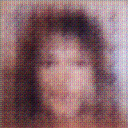
\includegraphics[width=150px]{500_fake_images/samples_5_342.png}%
\caption{A Close Up Of A Person Wearing A Tie}%
\end{figure}

%
\end{document}